\documentclass[UTF-8]{article}
\usepackage{amsmath}
\usepackage{amssymb}
\usepackage{float}
\usepackage{graphicx}
\usepackage{epstopdf}
\usepackage{inputenc}
\usepackage{geometry}
\usepackage{pgfplots} 
\usepackage{listings}
\usepackage{enumitem}
\usepackage{lipsum}  
\usepackage{color}
\usepackage[colorlinks=true, urlcolor=blue, linkcolor=blue]{hyperref}
\geometry{left=2.5cm,right=2.5cm,top=2.5cm,bottom=2.5cm}

\definecolor{codegreen}{rgb}{0,0.6,0}
\definecolor{codegray}{rgb}{0.2,0.2,0.2}
\definecolor{codepurple}{rgb}{0.58,0,0.82}
\definecolor{backcolour}{rgb}{0.95,0.95,0.952}

\lstdefinestyle{mystyle}{
	backgroundcolor=\color{backcolour},   
	commentstyle=\color{codegreen},
	keywordstyle=\color{blue},
	numberstyle=\tiny\color{codegray},
	stringstyle=\color{codepurple},
	basicstyle=\ttfamily\footnotesize,
	breakatwhitespace=false,         
	breaklines=true,                 
	captionpos=b,                    
	keepspaces=true,                 
	numbers=left,                    
	numbersep=5pt,                  
	showspaces=false,                
	showstringspaces=false,
	showtabs=false,                  
	tabsize=2,
	% linewidth=1.185\linewidth,
	% resetmargins=true,
	% xleftmargin=-1cm,
	% xrightmargin=0.085\textwidth,
	prebreak = \raisebox{0ex}[0ex][0ex]{\ensuremath{\hookleftarrow}}
}

\lstset{style=mystyle}
\pgfplotsset{compat=1.18}
\parindent 0cm

\title{High Performance Computing Proseminar 2024 \\
    \large Assignment 3} %exchange for assignment number

\author{Stefan Wagner \& Sebastian Bergner\\Team: Planning Desaster}
\begin{document}
    
    \maketitle
    
    The goal of this assignment is to extend the heat stencil application and measure its performance. 
    
    \section*{Exercise 1}
    This exercise consists in extending the heat stencil application of Assignment 2 to two dimensions. 
    \newline
    \begin{itemize}
    	\item Extend the heat stencil application to the two-dimensional case and name it 
            \texttt{heat\_stencil\_2D}. Provide a sequential and an MPI implementation. Try to make your implementation as efficient as possible, also with regard to code readability.
\begin{lstlisting}
01\_heat\_stencil\_2D/src/heat\_stencil\_2D\_seq.c
01\_heat\_stencil\_2D/src/heat\_stencil\_2D\_par\_blocking.c
\end{lstlisting}
    	\item Run your programs with multiple problem and machine sizes and measure speedup and 
            efficiency. Consider using strong scalability, weak scalability, or both. Justify your choice.
            \begin{itemize}
                \item \textbf{Strong vs Weak Scaling}:
                \begin{itemize}
                    \item In \textbf{strong scaling}, the problem size remains constant while the number of processors is increased. This allows us to measure how much faster the computation becomes with additional resources.
                    \item In \textbf{weak scaling}, the number of processors and the problem size are expanded proportionally, ensuring that each processor continues to handle the same amount of work.
                    \item We use \textbf{strong scaling} because our focus is on improving the performance of a fixed problem size. In practical applications like the 2D heat stencil, the problem size often remains constant, and our goal is to minimize the computation time by utilizing more processors. Strong scaling allows us to evaluate how efficiently the application distributes a fixed workload across multiple processors, which is the key to enhancing performance in real-world scenarios.
                \end{itemize}
                \item \textbf{Strong scaling speedup \& efficiency}:\\
                \[
                    S(p) = \frac{T_s}{T_p} \quad\quad E(p) = \frac{S(p)}{p}
                \]
                where $T_s$ is the sequential execution time and $T_p$ is the paralell execution time with $p$ processors.
            \end{itemize}
            \newpage
    	\item Illustrate the data in appropriate figures and discuss them. What can you observe?\\\\
            As demonstrated in Table \ref{table:01_measurements_table} and Figure \ref{fig:01_measurements_wall_time}, the parallel blocking version consistently outperforms the sequential version across all configurations and problem sizes. However, as problem sizes increase, while the speedup improves significantly, the efficiency declines, as illustrated in Figures \ref{fig:01_measurements_speedup} and \ref{fig:01_measurements_efficiency}.

            \begin{table}[H]
                \begin{tabular}{|lllll|}
\hline
\multicolumn{5}{|c|}{\textbf{Results of 2D Heat Stencil Execution}} \\ \hline
\multicolumn{1}{|c|}{\textbf{Impl/Ranks}} & \multicolumn{4}{c|}{\textbf{Problem Size}} \\ \hline
\multicolumn{1}{|c|}{\textbf{}} & \multicolumn{4}{c|}{\textbf{384}} \\ \hline
\multicolumn{1}{|l|}{} & \multicolumn{1}{c|}{$\mu$ [s]} & \multicolumn{1}{c|}{$\sigma$ [s]} & \multicolumn{1}{c|}{S(p)} & \multicolumn{1}{c|}{E(p)} \\ \hline
\multicolumn{1}{|l|}{seq/1}  & \multicolumn{1}{r|}{54.70} & \multicolumn{1}{r|}{41.33} & \multicolumn{1}{r|}{1.00} & \multicolumn{1}{r|}{1.00}  \\ \hline
\multicolumn{1}{|l|}{par\_block/6}  & \multicolumn{1}{r|}{43.36} & \multicolumn{1}{r|}{49.53} & \multicolumn{1}{r|}{1.26} & \multicolumn{1}{r|}{0.21}  \\ \hline
\multicolumn{1}{|l|}{par\_non\_block/6}  & \multicolumn{1}{r|}{42.34} & \multicolumn{1}{r|}{49.14} & \multicolumn{1}{r|}{1.29} & \multicolumn{1}{r|}{0.22}  \\ \hline
\end{tabular}

                \caption{2D Heat Stencil Measurement Results}
                \label{table:01_measurements_table}
            \end{table}
            \begin{figure}[H]
                \centering
                \includegraphics[width=0.8\linewidth]{01/measurements_wall_time.png}
                \caption{2D Heat Stencil: Wall Time}
                \label{fig:01_measurements_wall_time}
            \end{figure}
            \begin{figure}[H]
                \centering
                \includegraphics[width=0.8\linewidth]{01/measurements_speedup.png}
                \caption{2D Heat Stencil: Speedup}
                \label{fig:01_measurements_speedup}
            \end{figure}
            \begin{figure}[H]
                \centering
                \includegraphics[width=0.8\linewidth]{01/measurements_efficiency.png}
                \caption{2D Heat Stencil: Efficiency}
                \label{fig:01_measurements_efficiency}
            \end{figure}
            

    	\item Measure and illustrate one domain-specific and one domain-inspecific performance 
            metric. What can you observe?
            \begin{itemize}
                \item \textbf{Heat Propagation Updates per Second}\\
                Heat propagation updates per second serve as the domain-specific performance metric. This metric tracks how many updates to the heat values are performed per second during the simulation, providing a direct measure of the algorithm's efficiency in propagating heat across the grid. The number of updates is inherently linked to both the grid size and the number of iterations, making it a key indicator of computational performance.\\\\
                As illustrated in Figure \ref{fig:01_measurements_calc_sec}, the parallel blocking version consistently outperforms the sequential version across all configurations and problem sizes, as expected.
                \begin{figure}[H]
                    \centering
                    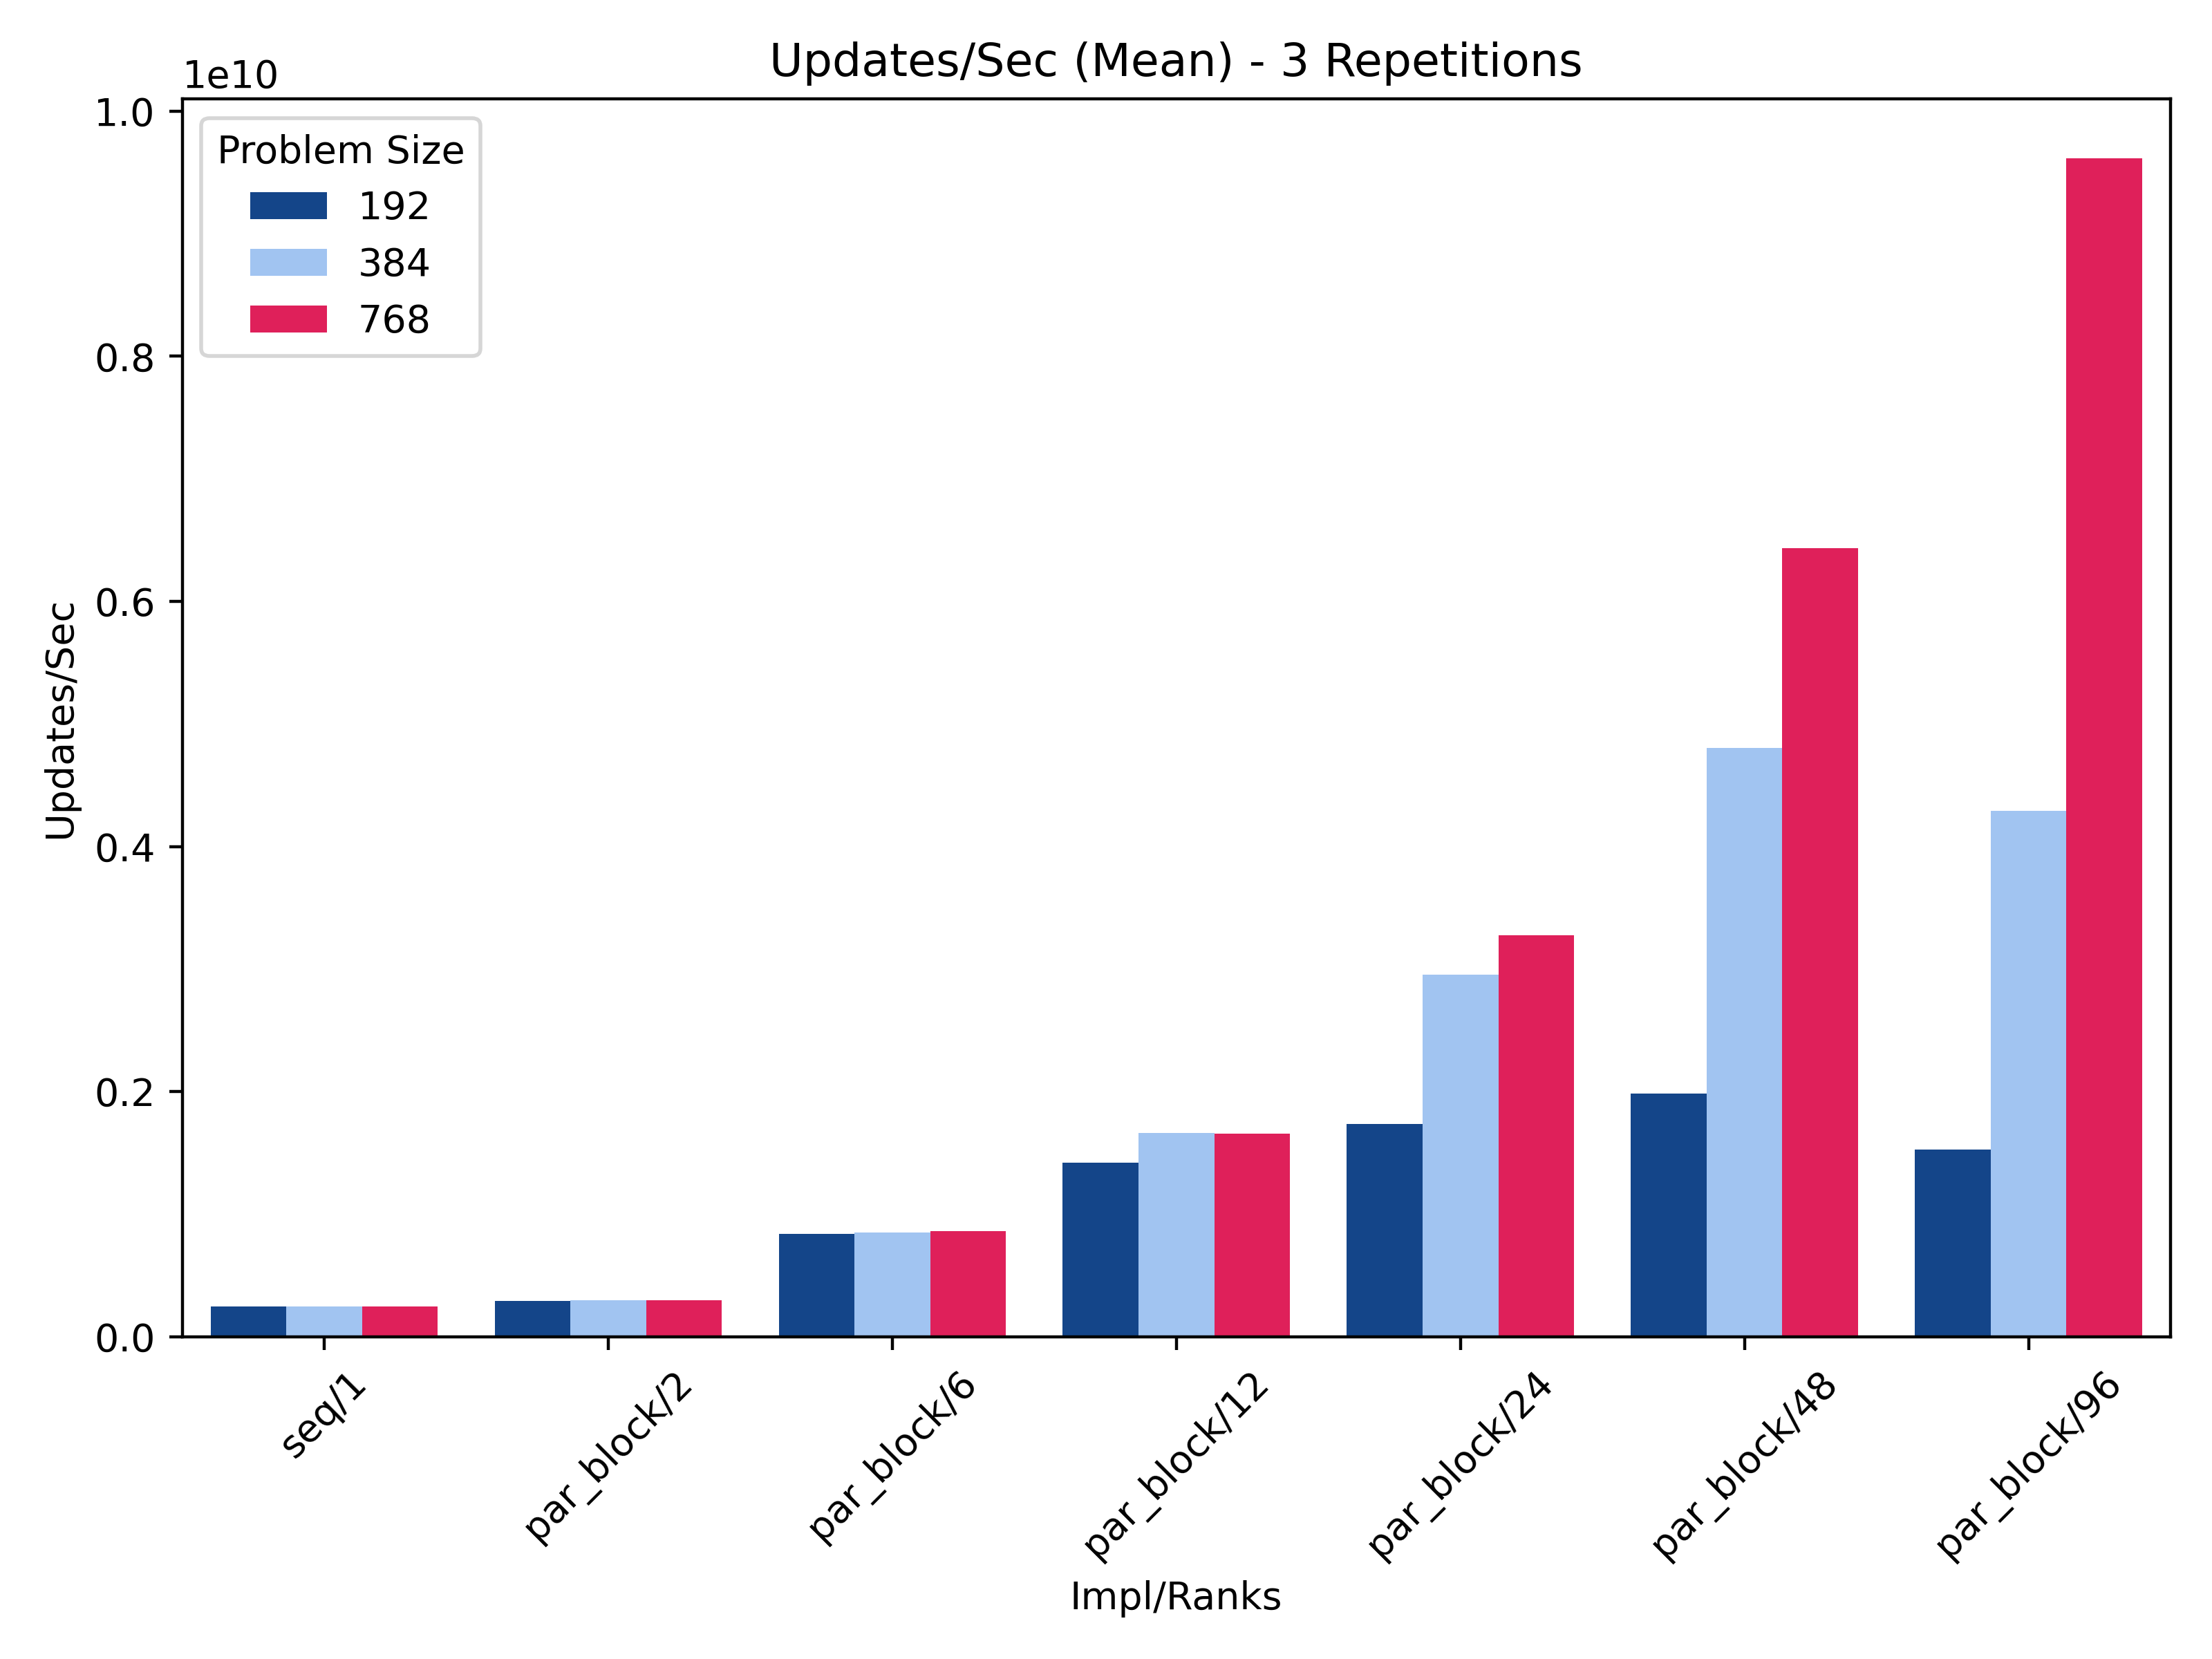
\includegraphics[width=0.8\linewidth]{01/measurements_calc_sec.png}
                    \caption{2D Heat Stencil: Updates/Sec}
                    \label{fig:01_measurements_calc_sec}
                \end{figure}
                
                \item \textbf{Wall Time}\\
                Wall time is used as the non-domain-specific performance metric. It captures the total computational time required by the algorithm, offering insight into the overall efficiency of the simulation. This metric is particularly valuable for evaluating how long the algorithm takes to complete for different problem sizes or configurations. Refer to the data in Table \ref{table:01_measurements_table} and the corresponding visualization in Figure \ref{fig:01_measurements_wall_time}.
            \end{itemize}
    	\item How can you verify the correctness of your applications?
            \begin{itemize}
                \item \textbf{Sequential Version}:\\
                To verify the correctness of the sequential 2D version, we applied the same verification checks used for the 1D version, ensuring that the output remained consistent across multiple executions and different problem sizes. We confirmed that the 2D output was correct based on our understanding of how it should appear in 2D, informed by the results from the 1D output.
                \item \textbf{Parallel Version}:\\
                To verify the correctness of the parallel applications, we compared the output of the parallel implementation with that of the sequential version. We ensured that both produced identical results across multiple executions. By running tests with different problem sizes and configurations, we confirmed that the parallel application consistently matched the sequential output, demonstrating the correctness of the parallelization.                
            \end{itemize}
    	\item Insert the wall times for the sequential version and for 96 cores for N=768x768 and T=N*100 into the comparison spreadsheet: \href{https://docs.google.com/spreadsheets/d/1p6d9F12EtykmI2-7MnHkg0U15UAtaCvWz8Ip92ZEsWo}{Docs}
    \end{itemize}

    \newpage
    \section*{Exercise 2}
    
    This exercise consists in comparing blocking and non-blocking communication for the heat stencil applications. 
    \newline
    \begin{itemize}
    	\item Provide an MPI implementation for the 1D and 2D heat stencil that uses non-blocking 
            communication. If you already implemented a non-blocking version, provide a blocking version, but ensure the non-blocking version works as described below.
\begin{lstlisting}
02_heat_stencil_blocking_vs_non_blocking/1D/src/heat_stencil_1D_seq.c
02_heat_stencil_blocking_vs_non_blocking/1D/src/heat_stencil_1D_par_blocking.c
02_heat_stencil_blocking_vs_non_blocking/1D/src/heat_stencil_1D_par_non_blocking.c
02_heat_stencil_blocking_vs_non_blocking/2D/src/heat_stencil_2D_seq.c
02_heat_stencil_blocking_vs_non_blocking/2D/src/heat_stencil_2D_par_blocking.c
02_heat_stencil_blocking_vs_non_blocking/2D/src/heat_stencil_2D_par_non_blocking.c
\end{lstlisting}
    	\item Structure your program such that you 1) start a non-blocking ghost cell exchange, 2) 
            compute the inner cells which do not require the result of the ghost cell exchange, 3) block until the ghost cell exchange has finished, and 4) compute the remaining cells.
    	\item Run your programs with multiple problem and machine sizes and compare both versions.
            \begin{table}[H]
                \hspace{-2cm}
                \begin{tabular}{|lllll|}
\hline
\multicolumn{5}{|c|}{\textbf{Results of 2D Heat Stencil Execution}} \\ \hline
\multicolumn{1}{|c|}{\textbf{Impl/Ranks}} & \multicolumn{4}{c|}{\textbf{Problem Size}} \\ \hline
\multicolumn{1}{|c|}{\textbf{}} & \multicolumn{4}{c|}{\textbf{384}} \\ \hline
\multicolumn{1}{|l|}{} & \multicolumn{1}{c|}{$\mu$ [s]} & \multicolumn{1}{c|}{$\sigma$ [s]} & \multicolumn{1}{c|}{S(p)} & \multicolumn{1}{c|}{E(p)} \\ \hline
\multicolumn{1}{|l|}{seq/1}  & \multicolumn{1}{r|}{54.70} & \multicolumn{1}{r|}{41.33} & \multicolumn{1}{r|}{1.00} & \multicolumn{1}{r|}{1.00}  \\ \hline
\multicolumn{1}{|l|}{par\_block/6}  & \multicolumn{1}{r|}{43.36} & \multicolumn{1}{r|}{49.53} & \multicolumn{1}{r|}{1.26} & \multicolumn{1}{r|}{0.21}  \\ \hline
\multicolumn{1}{|l|}{par\_non\_block/6}  & \multicolumn{1}{r|}{42.34} & \multicolumn{1}{r|}{49.14} & \multicolumn{1}{r|}{1.29} & \multicolumn{1}{r|}{0.22}  \\ \hline
\end{tabular}

                \caption{1D Heat Stencil Measurement Results}
                \label{table:02_1D_measurements_table}
            \end{table}
            \begin{figure}[H]
                \centering
                \includegraphics[width=0.8\linewidth]{02/1D/measurements_wall_time.png}
                \caption{1D Heat Stencil: Wall Time}
                \label{fig:02_1D_measurements_wall_time}
            \end{figure}
            \begin{figure}[H]
                \centering
                \includegraphics[width=0.8\linewidth]{02/1D/measurements_speedup.png}
                \caption{1D Heat Stencil: Speedup}
                \label{fig:02_1D_measurements_speedup}
            \end{figure}
            \begin{figure}[H]
                \centering
                \includegraphics[width=0.8\linewidth]{02/1D/measurements_efficiency.png}
                \caption{1D Heat Stencil: Efficiency}
                \label{fig:02_1D_measurements_efficiency}
            \end{figure}

            \begin{table}[H]
                \begin{tabular}{|lllll|}
\hline
\multicolumn{5}{|c|}{\textbf{Results of 2D Heat Stencil Execution}} \\ \hline
\multicolumn{1}{|c|}{\textbf{Impl/Ranks}} & \multicolumn{4}{c|}{\textbf{Problem Size}} \\ \hline
\multicolumn{1}{|c|}{\textbf{}} & \multicolumn{4}{c|}{\textbf{384}} \\ \hline
\multicolumn{1}{|l|}{} & \multicolumn{1}{c|}{$\mu$ [s]} & \multicolumn{1}{c|}{$\sigma$ [s]} & \multicolumn{1}{c|}{S(p)} & \multicolumn{1}{c|}{E(p)} \\ \hline
\multicolumn{1}{|l|}{seq/1}  & \multicolumn{1}{r|}{54.70} & \multicolumn{1}{r|}{41.33} & \multicolumn{1}{r|}{1.00} & \multicolumn{1}{r|}{1.00}  \\ \hline
\multicolumn{1}{|l|}{par\_block/6}  & \multicolumn{1}{r|}{43.36} & \multicolumn{1}{r|}{49.53} & \multicolumn{1}{r|}{1.26} & \multicolumn{1}{r|}{0.21}  \\ \hline
\multicolumn{1}{|l|}{par\_non\_block/6}  & \multicolumn{1}{r|}{42.34} & \multicolumn{1}{r|}{49.14} & \multicolumn{1}{r|}{1.29} & \multicolumn{1}{r|}{0.22}  \\ \hline
\end{tabular}

                \caption{2D Heat Stencil Measurement Results}
                \label{table:02_2D_measurements_table}
            \end{table}
            \begin{figure}[H]
                \centering
                \includegraphics[width=0.8\linewidth]{02/2D/measurements_wall_time.png}
                \caption{2D Heat Stencil: Wall Time}
                \label{fig:02_2D_measurements_wall_time}
            \end{figure}
            \begin{figure}[H]
                \centering
                \includegraphics[width=0.8\linewidth]{02/2D/measurements_speedup.png}
                \caption{2D Heat Stencil: Speedup}
                \label{fig:02_2D_measurements_speedup}
            \end{figure}
            \begin{figure}[H]
                \centering
                \includegraphics[width=0.8\linewidth]{02/2D/measurements_efficiency.png}
                \caption{2D Heat Stencil: Efficiency}
                \label{fig:02_2D_measurements_efficiency}
            \end{figure}
            
    	\item Insert wall time for 96 cores for N=768x768 and T=N*100 into the comparison spreadsheet: \href{https://docs.google.com/spreadsheets/d/1p6d9F12EtykmI2-7MnHkg0U15UAtaCvWz8Ip92ZEsWo}{Docs}
    \end{itemize}
\end{document}